\documentclass[12pt]{extreport}
\usepackage[utf8]{inputenc}
\usepackage[english]{babel}
\usepackage[T1]{fontenc}
\usepackage{graphicx, color}
\usepackage{float}
\usepackage{subcaption}
\usepackage{url}
\usepackage{amsfonts}
\usepackage{amsmath}
\usepackage[a4paper,margin=2cm]{geometry}
\usepackage[authoryear]{natbib}
%\usepackage{refcheck}
\usepackage{hyperref}
\hypersetup{
    colorlinks,
    citecolor=black,
    filecolor=black,
    linkcolor=black,
    urlcolor=black
}

\begin{document}

\begin{titlepage}

\newcommand{\HRule}{\rule{\linewidth}{0.5mm}} % Defines a new command for the horizontal lines, change thickness here
\center % Center everything on the page
 
%----------------------------------------------------------------------------------------
%	HEADING SECTIONS
%----------------------------------------------------------------------------------------


\includegraphics[width=\linewidth]{assets/logos/uvaENG.eps}\\[2.5cm]
\textsc{\Large MSc Artificial Intelligence}\\[0.2cm]
\textsc{\Large Master Thesis}\\[0.5cm]

%----------------------------------------------------------------------------------------
%	TITLE SECTION
%----------------------------------------------------------------------------------------

\HRule \\[0.4cm]
{ \huge \bfseries Detecting and Addressing Change in Machine Learning Data Pipelines}\\[0.4cm] % Title of your document
\HRule \\[0.5cm]
 
%----------------------------------------------------------------------------------------
%	AUTHOR SECTION
%----------------------------------------------------------------------------------------

by\\[0.2cm]
\textsc{\Large Bogdan Floris}\\[0.2cm] %you name
12140910\\[1cm]


%----------------------------------------------------------------------------------------
%	DATE SECTION
%----------------------------------------------------------------------------------------

{\Large \today}\\[1cm] % Date, change the \today to a set date if you want to be precise

Number of credits: 48 ECTS\\ %
November 2019 - July 2020\\[1cm]%

%----------------------------------------------------------------------------------------
%	COMMITTEE SECTION
%----------------------------------------------------------------------------------------
\noindent
\begin{minipage}[t]{0.4\textwidth}
\begin{flushleft} \large
\emph{Supervisors:} \\
prof. dr. Paul \textsc{Groth}\\
dr. Jakub \textsc{Zavrel}
\end{flushleft}
\end{minipage}
\begin{minipage}[t]{0.4\textwidth}
\begin{flushright} \large
\emph{Assessor:} \\
prof. dr. Paul \textsc{Groth}\\
\end{flushright}
\end{minipage}\\[2cm]

%----------------------------------------------------------------------------------------
%	LOGO SECTION
%----------------------------------------------------------------------------------------

%\framebox{\rule{0pt}{2.5cm}\rule{2.5cm}{0pt}}\\[0.5cm]
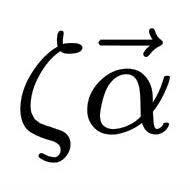
\includegraphics[width=2.5cm]{assets/logos/zeta-alpha-logo.jpg}\\ % Include a department/university logo - this will require the graphicx package
\textsc{\large Zeta Alpha Vector}\\[1.0cm] % 
 
%----------------------------------------------------------------------------------------

\vfill % Fill the rest of the page with whitespace

\end{titlepage}

\chapter*{Abstract}

Insert abstract here.

\chapter*{Acknowledgements}

Insert the acknowledgements here.

\tableofcontents

\listoffigures

\listoftables

\chapter{Introduction}

\begin{itemize}
    \item General introduction to the field (Machine Learning, NLP)
    \item Small overview of the topic being researched in this paper
    \item Why this topic?
    \item Description of the framework \ref{fig:framework}
\end{itemize}

\begin{figure}[h!]
\centering
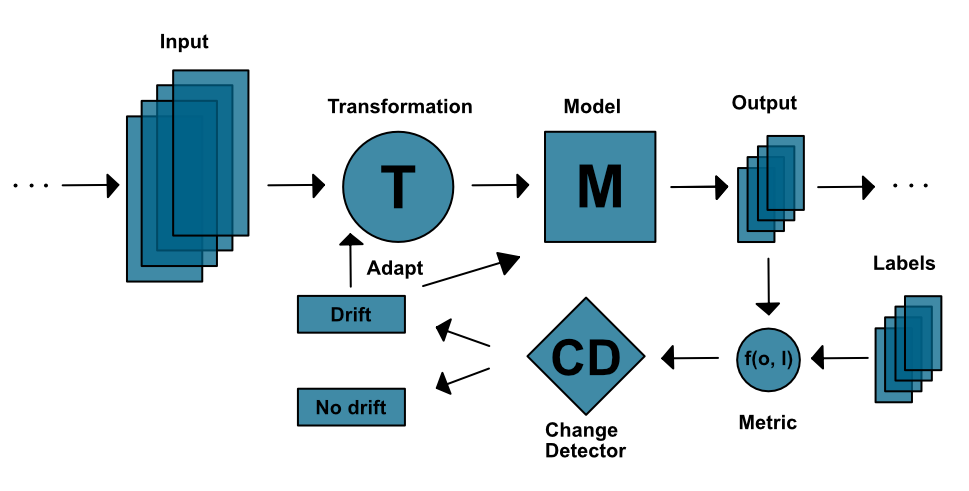
\includegraphics[width=\linewidth]{assets/introduction/framework.png}
\caption{General overview of the architecture}
\label{fig:framework}
\end{figure}

\section{Research Questions}

The main goal of this thesis is to develop a general framework in which machine learning models that are part of streaming data pipelines can detect changes in their output distribution and adapt to them accordingly, while also successfully applying this framework on a specific natural language processing use case that is of interest to Zeta Alpha Vector. This comprehensive topic will be tackled with the following research questions, covered below together with a short description for each question.

\paragraph*{How can we quickly detect that the output distribution of a model has changed given a continuous stream of data, and then report on the degree of change?} Insert description of this research question

\paragraph*{Given that a change was detected, how can we adapt the model efficiently such that the performance is the same as it previously was before the change?} Insert overall description of the question here, them break it down to the two other questions:
\begin{itemize}
    \item \textbf{Given a small change (gradual drift or small abrupt drift), can we adapt the model by feeding it with a few examples, compared to retraining it from scratch?} Description about this subquestion.
    \item \textbf{Given a big change (big abrupt drift), can we adapt the model by finding a mapping between the old outputs and the new ones which is less expensive to compute than retraining the model from scratch?} Description about this subquestion
\end{itemize}

\chapter{Background}

In this chapter, we introduce the background needed to support the work done in this thesis. First, we give a brief overview of the framework in which change can occur, a data pipeline, and present the concept of online learning. Then we go into more details about the work that has been done on detecting change in this framework, explaining concept drift. Finally, we also present a small overview of the agent of change that acts of the pipeline, word embeddings.

\section{Streaming Data Pipelines and Online Learning}

Since the turn of the century, as memory became increasingly cheaper and the internet more and more widespread throughout the world, companies have started to collect enormous amounts of data. According to \cite{big-data-beginning-future}, the amount of data doubles every two years, with the trend showing no signs of stopping. This phenomenon has given birth to the field of big data, which aims to develop techinques to process and analyze data that is too large or complex for traditional data analysis tools (\cite{wiki:big-data}). Big data has been forcing companies to slowly move away from traditional machine learning algorithms because these work in an offline setting. In offline machine learning, all data is available from the start and can be fed as batches to train the model, with each sample being used more than once potentially. This method is usually infeasible in the context of big data, so \cite{advances-knowledge-discovery} have proposed a few requirements for these large scale machine learning data pipelines:

\begin{itemize}
    \item The training of a model should be done continuously and only on blocks of data or separate samples.
    \item Each sample should only be used once to train the model.
    \item We should assume that the samples are not stored after they have been seen by the model.
\end{itemize}

The third requirement can be relaxed in practice depending on how much storage is available, and most large scale data pipelines usually store at least a recent window of the data.

Online learning is the type of data analysis usually deployed in streaming data pipelines and is defined as a learner which attemps to solve an online decision task by fitting a model to a sequence of data that arrives one at a time (\cite{onlinelearning}). This is in contrast to offline (batch) machine learning, which requires that all data be present when training the model. The main advantage of online learning is that it is highly scalable in terms of both computing power and storage, which is suitable for big data, but it is also not as performant as batch learning since it only sees the samples once and not in an arbitrary order. According to \cite{onlinelearning}, there are three types of online learning:

\begin{itemize}
    \item Supervised online learning where feedback is immediately available.
    \item Online learning with limited feedback (e.g. only a few samples also have labels).
    \item Unsupervised online learning where there is no feedback.
\end{itemize}

The work done in this thesis will mainly focus on supervised online learning, while briefly touching on how a lack of supervision could be handled.

\section{Concept drift} \label{concept-drift}

\subsection{Definition}

Online data pipelines should in theory operate endlessly after being deployed, but the nature of data in general makes the environment in which they operate dynamic. One example would be the change in the distribution of the data samples that arrive at the pipeline. This phenomenon is known in theory as concept drift (\cite{survey-concept-drift}). Take for example a set of data $X$ with a target variable $y$, where we are trying to learn a function $f$, such that $y = f(X)$. Predictions models usually require and assume stationarity in the data (\cite{Heng_Wang_2015}), so if we make this assumption we can fit $f$ once and assume that it works for all subsequent data coming to the pipeline. In practice, however, it might happen that the distribution of $X$ changes, and so the relationship between $X$ and $y$ also does, which makes our estimate of $f$ outdated.

We can use the framework (\ref{fig:framework}) to formally define the problem addressed in this thesis as a concept drift issue. Let $W$ be the initial, unprocessed dataset (which will be described in \ref{wos}) with labels $\mathbb{C}$ that denote classes, $\mathbb{T}$ a set of transformation functions (for example a function that extracts features out of the initial dataset), and $X$ the transformed input $\forall i: x_i = t(w_i)$, where $t \in \mathbb{T}$. We can then use Bayesian Decision Theory (\cite{pattern-classification}) to state the classification task. The probability $P(c_k), c_k \in \mathbb{C}$ is known as the \emph{a priori} and reflects the probability that a samples belongs to class $c_k$. The probability $P(X|c_k)$ is known as the \emph{class conditional density function} and reflects the probability density of $X$ when class $c_k$ is known. When can use Bayes' Rule to solve for the \emph{posterior}:

\begin{equation}
    P(c_k|X) = \frac{P(X|c_k) P(c_k)}{P(X)}
\end{equation}

Concept drift occurs if for two time points $t_1$, $t_2$, where $t_2 > t_1$, $\exists x \in X: P_{t_1}(x|c_k) \neq P_{t_2}(x|c_k)$. For our purposes, we will assume that $W$ remains stationary and the distribution shift happens because of a change in the transformation functions $\mathbb{T}$, induced by the pipeline switching from transformation function to another.

\subsection{Concept drift types}

Concept drift is the shift in the distribution of the dataset as samples come to the pipeline, but of equal importance to both detection and overcoming change is the type of concept drift. \cite{survey-concept-drift} describe a few types of drift, but for all intents and purposes, we can distinguish between three types:

\begin{itemize}
    \item Big abrupt concept drift (figure \ref{fig:big-abrupt-drift}), which is signalled by a big instant change in the distribution that results in the model's accuracy degrading heavily.
    \item Small abrupt concept drift (figure \ref{fig:small-abrupt-drift}), which is signalled by a small instant change in the distrbution that results in the model's accuracy degrading just slighly.
    \item Gradual concept drift (figure \ref{fig:gradual-drift}), which is is signalled by small incremental changes in the distribution that in time have the same effect on the model as a big abrupt change but take a much longer time to occur.
\end{itemize}

\begin{figure}[ht!]
\centering
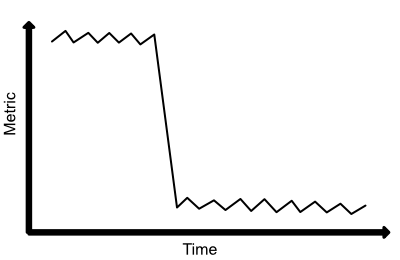
\includegraphics[width=0.6\linewidth]{assets/preliminaries/big-abrupt-drift.png}
\caption{Big abrupt concept drift}
\label{fig:big-abrupt-drift}
\end{figure}

\begin{figure}[ht!]
\centering
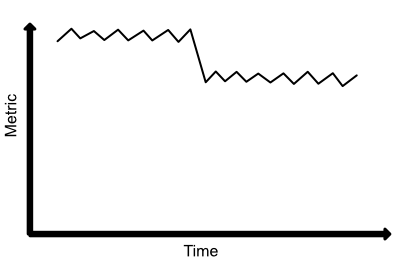
\includegraphics[width=0.6\linewidth]{assets/preliminaries/small-abrupt-drift.png}
\caption{Small abrupt concept drift}
\label{fig:small-abrupt-drift}
\end{figure}

\begin{figure}[ht!]
\centering
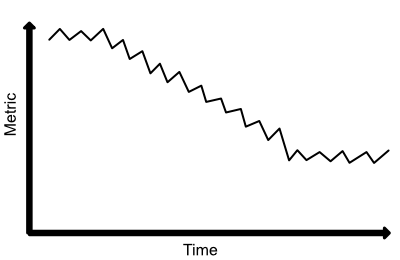
\includegraphics[width=0.6\linewidth]{assets/preliminaries/gradual-drift.png}
\caption{Gradual concept drift}
\label{fig:gradual-drift}
\end{figure}

As mentioned earlier, the type of concept drift encountered has an impact of both detecting and addressing change. As emphasized in the next section, there are quite a few algorithms that are used in practice to detect concept drift, and most of them are better at detecting a specfici type of drift, so there is no free lunch. As shown in the experiments in the next chapter, gradual drift is harder to detect and it's quite easy to trigger a false positive. When in comes to addressing change, there are again a few options from which to choose. For example, a fine tuning approach might work for a small abrupt drift, but doing it for a big abrupt drift is akin to retraining the model from scratch, something we would like to avoid.

\subsection{Concept drift detection algorithms}

While there has been ample research involved in detecting anomalies in data which is at rest (\cite{survey-outlier-detection} provides a nice overview of the methodologies employed in anomaly detection and \cite{there-and-back-again} comes with a data mining perspective on outlier detection), machine learning pipelines are anything but static. Data is continuously pushed through the system, so the metrics computed from the models’ outputs are adjusted endlessly. Moreover, this uninterrupted flow in the system makes storing all these metrics infeasible, so the pipeline must be able to make a decision on whether or not a concept drift occurred based only on the most recent samples.

\cite{detecting-change-in-data-streams} wrote one of the pioneering papers on detecting change in data streams and came up with a novel solution that keeps two windows for the incoming stream and comapres the two using a new distance metric that proves to be a good indicator for the degree of change, as it was specifically designed with this in mind. Their method could be improved by using a different method for saving samples, like the space saving algorithm for detecting heavy hitters, as described in \cite{hierarchical-heavy-hitters}. \cite{onlineanomalydetection} uses more simple distance metrics like relative entropy and Pearson correlation, but the approach is tailored towards big data streams. ADWIN (\cite{adwin}) improves on \cite{detecting-change-in-data-streams} by making the size of the window adaptable, resizing it according to the rate of change observed from the data in the window itself. Two methods that are especially suited for detecting drift in classification tasks using metrics are DDM (\cite{ddm}) and EDDM (\cite{eddm}). Both of them are based on the estimated distribution of the distances between classification errors, but DDM is more suitable for abrupt drift, while EDDM is better for gradual drift. A more state of the art paper, \cite{hht}, presents a novel framework for hierarchical hypothesis testing, a concept drift detector named Hierarchical Linear Four Rates, which achieves great results on type I and II errors.

\subsection{Concept drift adaptation}

Concept drift adaptation is a newer topic of interest in the scientific community, but it is gaining more and more traction as models are becoming increasingly costly to retrain. \cite{hht} mentions that there are two different approaches to address concept drifts in streaming data. Continuing adaptation doesn’t include a concept drift detector, but assumes that the environment will change and either keeps updating the model parameters incrementally (\cite{adwin}), or learns an ensemble of models on different windows in the stream (\cite{incremental-learning-of-concept-drift}). Adaptation with drift detection actually employs a detector, which signals that a change has occurred and then makes a decision on which adaption technique to use based on the degree of change (\cite{concept-drift-detection-for-streaming-data}).

\section{Word embeddings}

We have mentioned in section \ref{concept-drift} that there is a set of transformation functions $\mathbb{T}$ that act as the agent of change on the initial dataset. The transformation agents that will be the main study of this thesis will be word embeddings, which have been main driving force behind the improvements in natural language understanding in the past decade (\cite{word-embedding-survey}). There were two main reasons that necessitated the development of word embeddings to represent text data:

\begin{itemize}
    \item Solutions before the introduction of word embeddings were based on bag of words, where a word was represented by the number of times it appeared in the text. The bag of words method had the clear disadvantage that it produced huge and sparse vectors, which were unsuitable for models. Word embeddings, on the other hand, produce short and dense vectors, which improves both the computational complexity and the understanding of the text (\cite{word-embedding-survey, word2vec}).
    \item Another issue with previous approaches was that the context of a word was not embedded into its representation in the vector space. Take for example these two sentences: \emph{I am writing in my notebook} and \emph{I am writing in my journal}. \emph{Notebook} and \emph{journal} have similar context and this should ideally be represented in their respective vectors. Their relationship is represented in theory by the cosine similarity (\cite{word2vec}): \begin{align}\text{similarity}(w_1, w_2) = \cos(\theta) = \frac{w_1 \dot w_2}{\lVert w_1 \rVert \lVert w_2 \rVert}\end{align}, where $\theta$ is the angle between the vectors of $w_1$ and $w_2$. The cosine similarity is no taken into account with the previous approaches, but word embeddings are optimized to improve it.
\end{itemize}

The breakthrough paper that introduced word embeddings to both the academic world and the industry was \texttt{word2vec} (\cite{word2vec}), which computes pre-trained word embeddings using a skip-gram model. Since then, the field has brought increasingly more improvements to non-contextual word embeddings, with some examples being \texttt{GloVe} (\cite{glove}) and \texttt{FastText} (\cite{fasttext}).

Recently, since the introduction of \texttt{BERT} (\cite{bert}) and ELMo (\cite{elmo}), the field has shifted to contextual word embeddings, which have brought with them great improvements to the state of art on a multitude of tasks (\cite{bert}). These embeddings are trained using a bi-directional transformer model by conditioning on both the left and right context of a word, thus creating better representations. Moreover, besides these different fundamental approaches to computing embeddings, each one of these approaches has dozens of pre-trained variations on different datasets or of different sizes (\cite{huggingface}). For example, \texttt{BERT} has seen variations that make it faster and cheaper computationally, like \texttt{DistilBERT} (\cite{distilbert}), or variations that make it work better for scientific text, like \texttt{SciBERT} (\cite{scibert}).

The trend is clear here. Every year, more and more papers come out that upend the state of the art and improve the natural language understanding models. The AI Index Report 2019 (\cite{aiindex2019}) mentions that the number of AI papers produced each year has increased by more than 9x since 1996, with a lot of them in the field of NLP. Thus, companies and AI practitioners have to constantly adapt to the new state of the art, plugging in new word representations to keep their models up to end. This ends up costing compute and development time, since the neural network models have become increasingly more complex from year to year as well (\cite{aiindex2019}). A data pipeline would be better if it could detect that a change in word embeddings has occurred and adapt itself to the new embedding space. Our work will focus on training a classification model using \texttt{BERT} (\cite{bert}), and then adapting the model to other embedding spaces, namely \texttt{SciBERT} (\cite{scibert}) and \texttt{DistilBERT} (\cite{distilbert}).

\chapter{Framework}

\section{Dataset}

\subsection{The Web of Science} \label{wos}

Short introduction to the Web of Science and why it's good to use because of the work done by Zeta Alpha.

\begin{figure}[ht!]
\centering
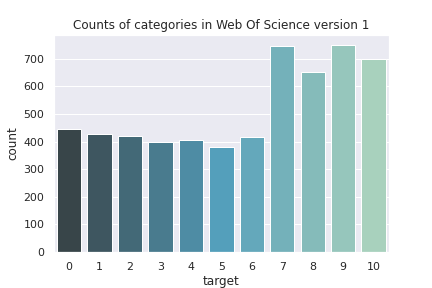
\includegraphics[width=0.8\linewidth]{assets/framework/wos_counts_1.png}
\caption{Web of Science counts for each label}
\label{fig:wos-1}
\end{figure}

Potentially add the two other variants of the Web of Science, but experiments need to be performed with those versions of the Web of Science too. That might not be worth it because analyzing the performance of the LSTM on the Web of Science is not the purpose of this thesis.

\subsection{Data stream}

Explain how the Web of Science was transformed into a data stream (batch sizes, adjustments, parameters, etc.).

\section{Models}

\subsection{Naive Bayes baseline}

\begin{itemize}
    \item Short introduction to the Naive Bayes model in general.
    \item Explain how the Naive Bayes model was adapted for our use case (things like picking the maximum over the sequence length axis in order to get a useable dataset for the model).
    \item Analyze the performance of the model and explain how the model is not robust enough.
\end{itemize}

\begin{figure}[ht!]
\centering
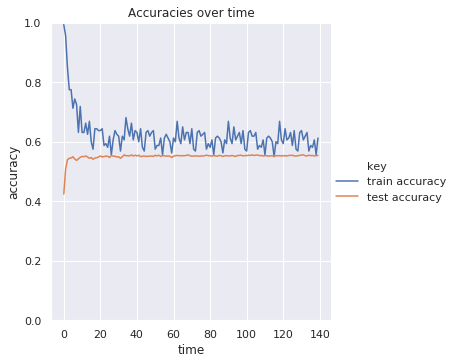
\includegraphics[width=0.8\linewidth]{assets/framework/nb_BERT_accuracy_holdout.png}
\caption{Naive Bayes accuracy over time using BERT embeddings}
\label{fig:nb-acc}
\end{figure}

Also show that the other metrics are performing on par with the accuracy for the test set using the following picture \ref{fig:nb-metrics}.

\begin{figure}[H]
\centering
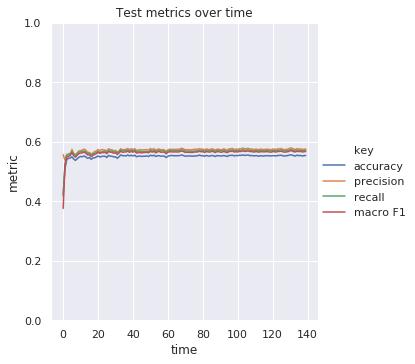
\includegraphics[width=0.8\linewidth]{assets/framework/nb_BERT_test_metrics_holdout.png}
\caption{Naive Bayes metrics over time for the test set}
\label{fig:nb-metrics}
\end{figure}

\subsection{LSTM}

\begin{itemize}
    \item Short introduction to LSTM models in general.
    \item Again, explanation of design choices made (how we solved the different sized sequences problem, and how we solved feeding it into a final fully connected layer for classification).
    \item Analyze the performance of the model and explain how the model is robust.
    \item Differences between the LSTM model and Naive Bayes one.
\end{itemize}

\begin{figure}[H]
\centering
\begin{subfigure}{.5\textwidth}
  \centering
  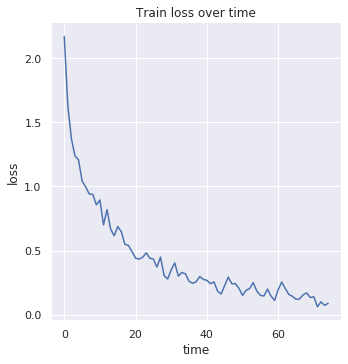
\includegraphics[width=.76\linewidth]{assets/framework/lstm_BERT_loss_holdout.png}
  \caption{Loss over time}
  \label{fig:lstm-loss}
\end{subfigure}%
\begin{subfigure}{.5\textwidth}
  \centering
  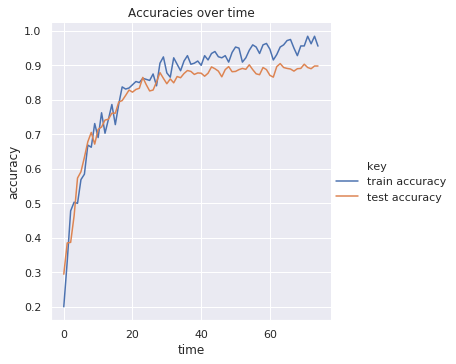
\includegraphics[width=\linewidth]{assets/framework/lstm_BERT_accuracy_holdout.png}
  \caption{Accuracy over time}
  \label{fig:lstm-acc}
\end{subfigure}
\caption{LSTM loss and accuracy over time using BERT embeddings}
\label{fig:lstm-loss-acc}
\end{figure}

Also show that the other metrics are performing on par with the accuracy for the test set using the following picture \ref{fig:lstm-metrics}.

\begin{figure}[H]
\centering
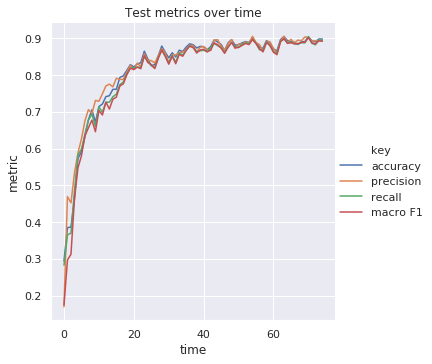
\includegraphics[width=0.8\linewidth]{assets/framework/lstm_BERT_test_metrics_holdout.png}
\caption{LSTM metrics over time for the test set}
\label{fig:lstm-metrics}
\end{figure}

\chapter{Detecting change}

\section{Experimental Setup}

\begin{itemize}
    \item Explain the different types of change detectors and their pros and cons.
    \item Explain how the experiments will be conducted: running a first stream using the embeddings that the model was trained while feeding the metrics to the change detector, then running another stream transformed using other embeddings and seeing how the model and the change detector react.
    \item We can change embeddings to produce a very small abrupt drift and change embeddings to produce a big abrupt drift.
    \item Testing for gradual drift will be done by adding random noise to the embeddings over time.
    \item Experiments will be run for both the Naive Bayes model and the LSTM model.
    \item We also need to differentiate between supervised computation of the metrics and unsupervised computation of the metrics.
    \item Mention how the sensitivity of the change detector needs to be adjusted for the unsupervised case.
    \item Mention that we show that the accuracy is 1 for the unsupervised trained model, but in practice we introduce randoms betwwen 0.9 and 1.
\end{itemize}

\section{Results}

This section will show the results for the change detection chapter without discussing the results.

\subsection{Naive Bayes model}

First show the results of changing embeddings. First BERT-DISTILBERT trying to provoke just a small abrupt drift, and then BERT-SCIBERT to provoke a big abrupt drift. We will show the supervised and the unsupervised side by side. Also explain the figures.

\begin{figure}[H]
\centering
\begin{subfigure}{.5\textwidth}
  \centering
  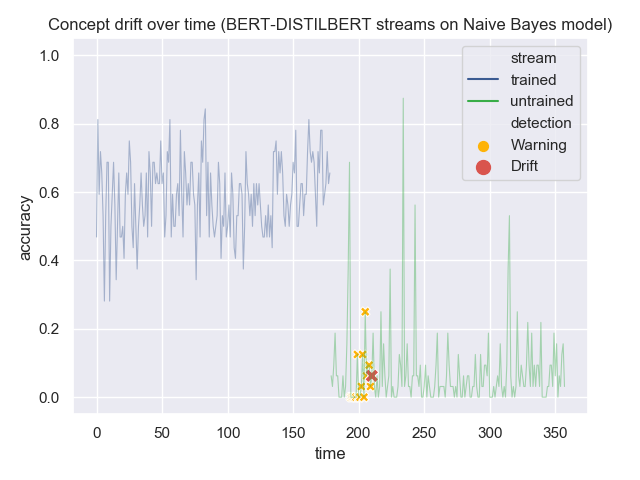
\includegraphics[width=\linewidth]{assets/detecting-change/diff_embed_nb_wos_1_BERT_DISTILBERT.png}
  \caption{Supervised change detection}
  \label{fig:nb-diff-embed-super-B-D}
\end{subfigure}%
\begin{subfigure}{.5\textwidth}
  \centering
  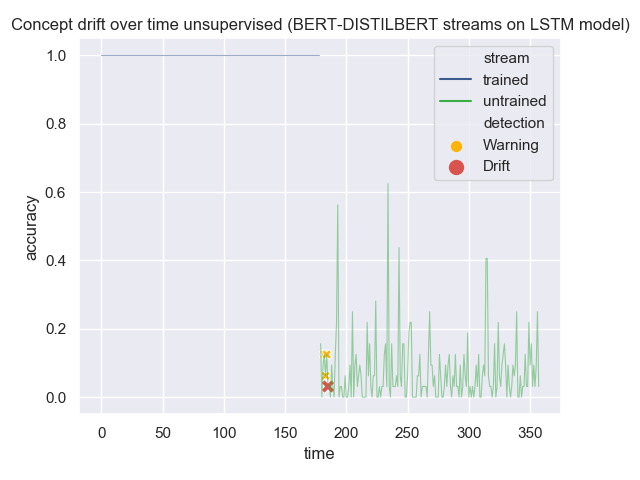
\includegraphics[width=\linewidth]{assets/detecting-change/diff_embed_nb_wos_1_BERT_DISTILBERT_unsupervised.png}
  \caption{Unsupervised change detection}
  \label{fig:nb-diff-embed-unsuper-B-D}
\end{subfigure}
\caption{Detecting change using different embeddings (BERT-DISTILBERT) in the Naive Bayes model}
\label{fig:nb-diff-embed-B-D}
\end{figure}

\begin{figure}[H]
\centering
\begin{subfigure}{.5\textwidth}
  \centering
  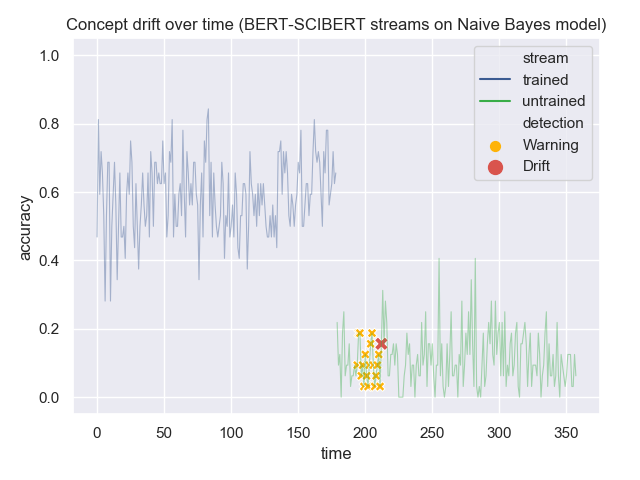
\includegraphics[width=\linewidth]{assets/detecting-change/diff_embed_nb_wos_1_BERT_SCIBERT.png}
  \caption{Supervised change detection}
  \label{fig:nb-diff-embed-super-B-S}
\end{subfigure}%
\begin{subfigure}{.5\textwidth}
  \centering
  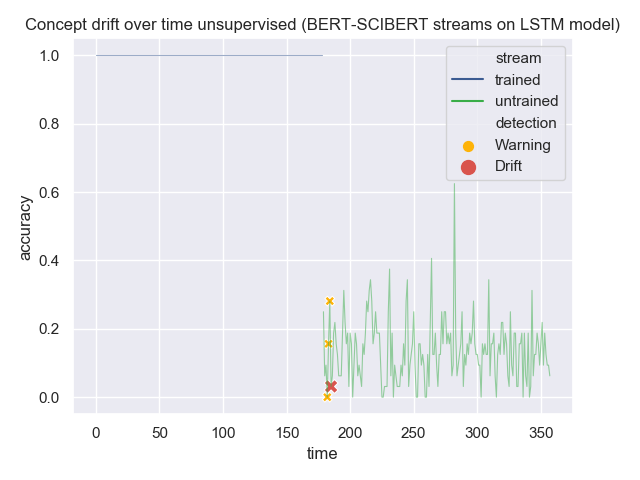
\includegraphics[width=\linewidth]{assets/detecting-change/diff_embed_nb_wos_1_BERT_SCIBERT_unsupervised.png}
  \caption{Unsupervised change detection}
  \label{fig:nb-diff-embed-unsuper-B-S}
\end{subfigure}
\caption{Detecting change using different embeddings (BERT-SCIBERT) in the Naive Bayes model}
\label{fig:nb-diff-embed-B-S}
\end{figure}

Next, we show the results of adding gradual noise to the Naive Bayes model.

\begin{figure}[H]
\centering
\begin{subfigure}{.5\textwidth}
  \centering
  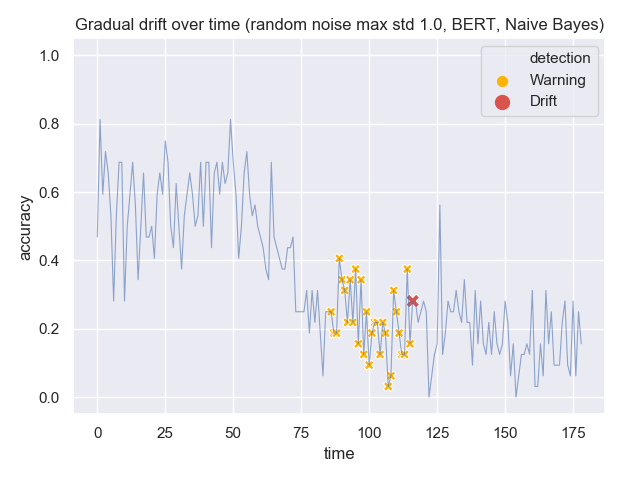
\includegraphics[width=\linewidth]{assets/detecting-change/gradual_noise_random_std_1_nb_wos_1_BERT.png}
  \caption{Gradual with std 1.0}
  \label{fig:nb-gradual-std-1}
\end{subfigure}%
\begin{subfigure}{.5\textwidth}
  \centering
  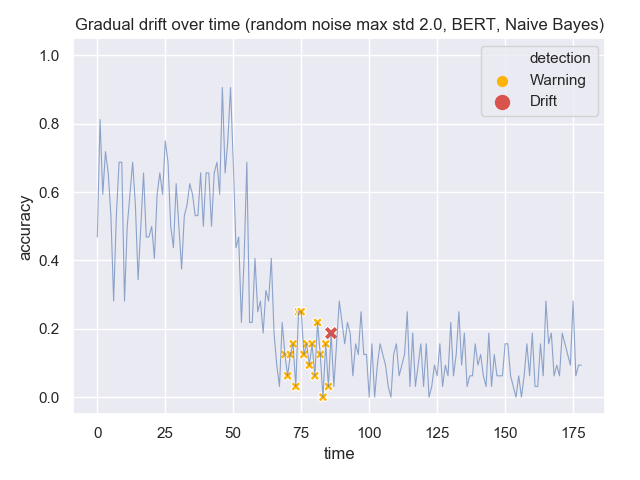
\includegraphics[width=\linewidth]{assets/detecting-change/gradual_noise_random_std_2_nb_wos_1_BERT.png}
  \caption{Gradual with std 2.0}
  \label{fig:nb-gradual-std-2}
\end{subfigure}
\begin{subfigure}{.5\textwidth}
  \centering
  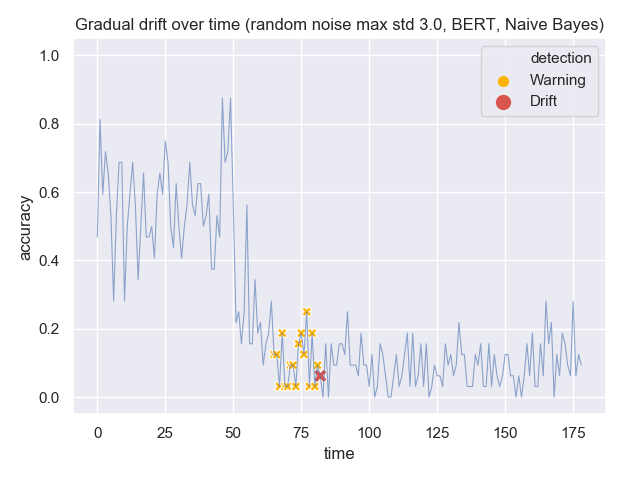
\includegraphics[width=\linewidth]{assets/detecting-change/gradual_noise_random_std_3_nb_wos_1_BERT.png}
  \caption{Gradual with std 3.0}
  \label{fig:nb-gradual-std-3}
\end{subfigure}
\caption{Detecting gradual change by adding random noise with different stds in the Naive Bayes model}
\label{fig:nb-gradual}
\end{figure}

\subsection{LSTM model}

Same things for the LSTM model.

\begin{figure}[H]
\centering
\begin{subfigure}{.5\textwidth}
  \centering
  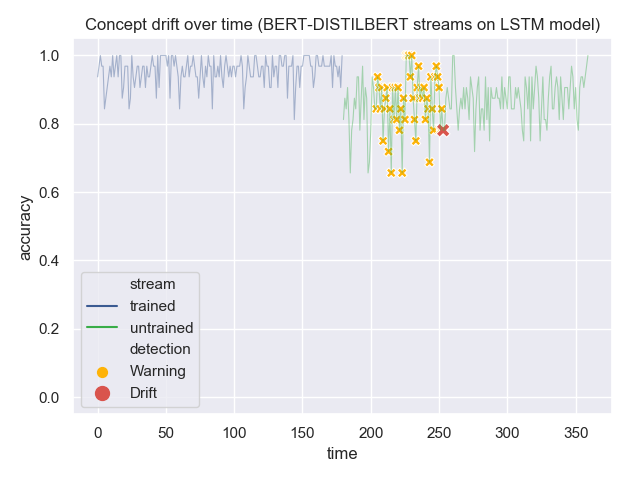
\includegraphics[width=\linewidth]{assets/detecting-change/diff_embed_lstm_wos_1_BERT_DISTILBERT.png}
  \caption{Supervised change detection}
  \label{fig:lstm-diff-embed-super-B-D}
\end{subfigure}%
\begin{subfigure}{.5\textwidth}
  \centering
  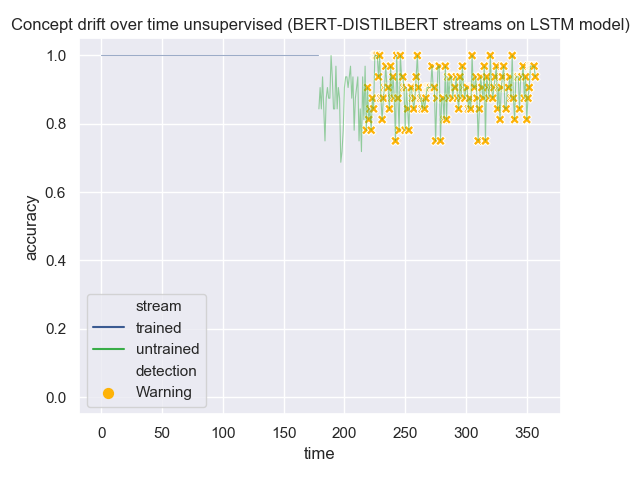
\includegraphics[width=\linewidth]{assets/detecting-change/diff_embed_lstm_wos_1_BERT_DISTILBERT_unsupervised.png}
  \caption{Unsupervised change detection}
  \label{fig:lstm-diff-embed-unsuper-B-D}
\end{subfigure}
\caption{Detecting change using different embeddings (BERT-DISTILBERT) in LSTM model}
\label{fig:lstm-diff-embed-B-D}
\end{figure}

\begin{figure}[H]
\centering
\begin{subfigure}{.5\textwidth}
  \centering
  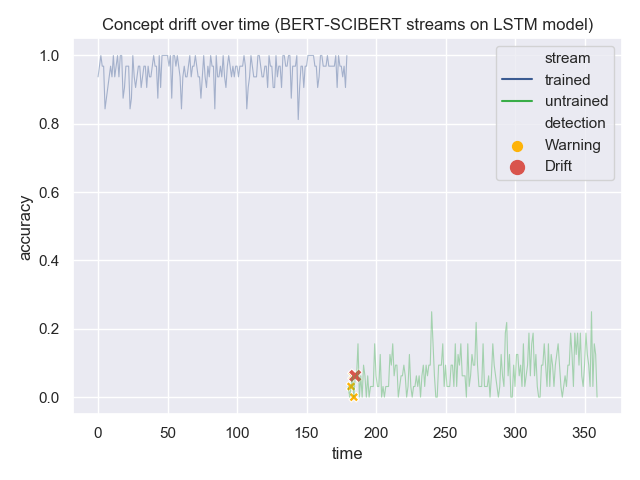
\includegraphics[width=\linewidth]{assets/detecting-change/diff_embed_lstm_wos_1_BERT_SCIBERT.png}
  \caption{Supervised change detection}
  \label{fig:lstm-diff-embed-super-B-S}
\end{subfigure}%
\begin{subfigure}{.5\textwidth}
  \centering
  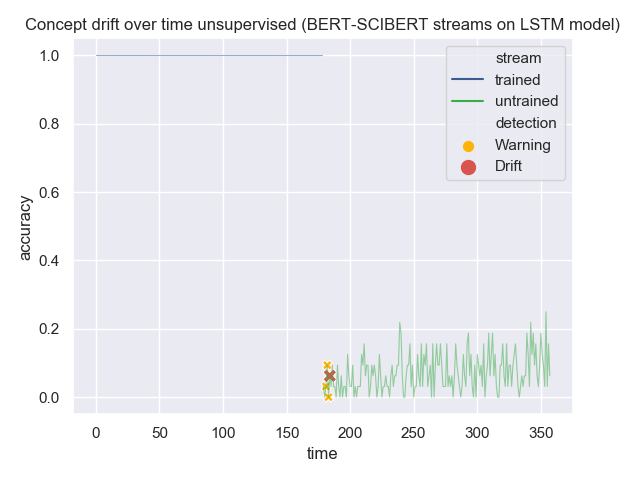
\includegraphics[width=\linewidth]{assets/detecting-change/diff_embed_lstm_wos_1_BERT_SCIBERT_unsupervised.png}
  \caption{Unsupervised change detection}
  \label{fig:lstm-diff-embed-unsuper-B-S}
\end{subfigure}
\caption{Detecting change using different embeddings (BERT-SCIBERT) in LSTM model}
\label{fig:lstm-diff-embed-B-S}
\end{figure}

Now gradual change for the LSTM model.

\begin{figure}[H]
\centering
\begin{subfigure}{.5\textwidth}
  \centering
  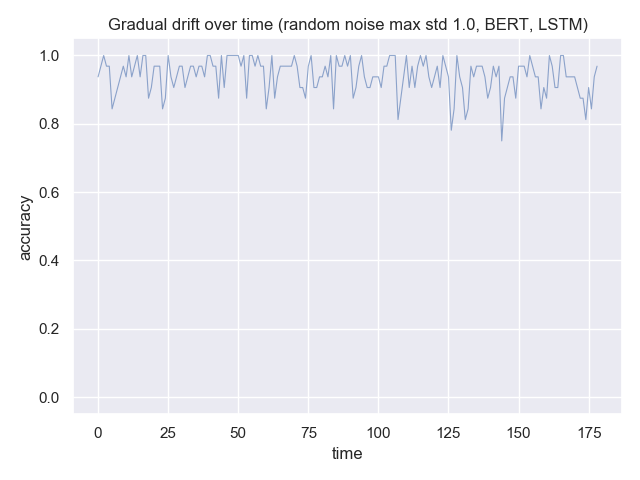
\includegraphics[width=\linewidth]{assets/detecting-change/gradual_noise_random_std_1_lstm_wos_1_BERT.png}
  \caption{Gradual with std 1.0}
  \label{fig:lstm-gradual-std-1}
\end{subfigure}%
\begin{subfigure}{.5\textwidth}
  \centering
  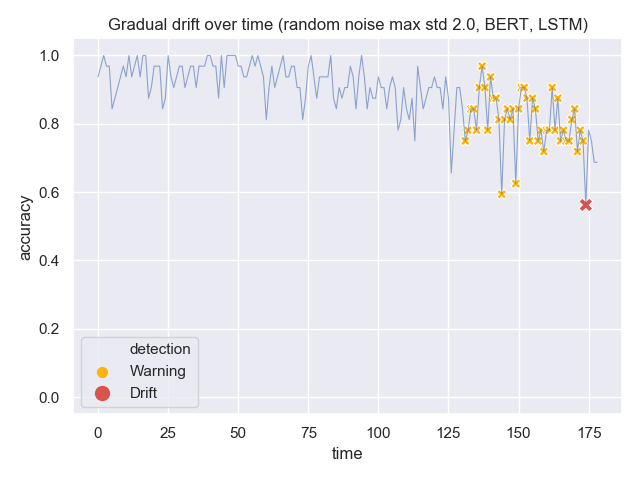
\includegraphics[width=\linewidth]{assets/detecting-change/gradual_noise_random_std_2_lstm_wos_1_BERT.png}
  \caption{Gradual with std 2.0}
  \label{fig:lstm-gradual-std-2}
\end{subfigure}
\begin{subfigure}{.5\textwidth}
  \centering
  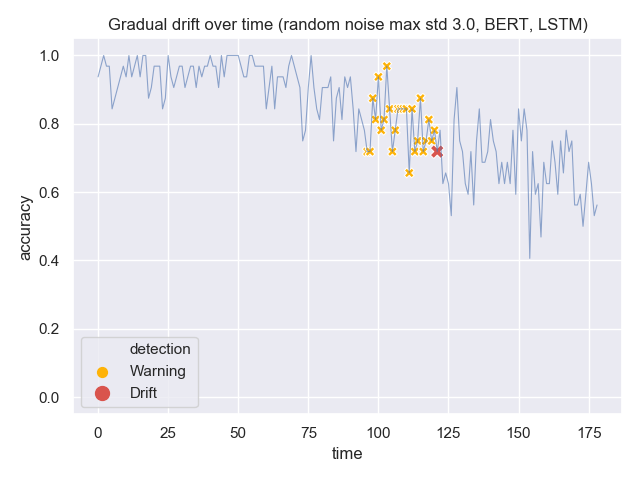
\includegraphics[width=\linewidth]{assets/detecting-change/gradual_noise_random_std_3_lstm_wos_1_BERT.png}
  \caption{Gradual with std 3.0}
  \label{fig:lstm-gradual-std-3}
\end{subfigure}
\caption{Detecting gradual change by adding random noise with different stds in the LSTM model}
\label{fig:lstm-gradual}
\end{figure}

\section{Discussion}

Main topics for discussion:
\begin{itemize}
    \item Difference in robustness between the LSTM model and the Naive Bayes model.
    \item Difference between supervised and unsupervised and how picking settings for the change detector and how we input values for accuracy to it (0.9-1) is very important and produces different results.
    \item How gradual noise affects the models
\end{itemize}

\chapter{Addressing change}

Two methods of addressing change:
\begin{itemize}
    \item For small abrupt drift or gradual drift, we can probably get away with feeding the model with a few batch and the accuracy should recover fairly fast.
    \item For big abrupt drift, one idea for adaptation is to create a mapping between the two different embedding sets.
\end{itemize}

Also mention that adaptation is useful only for the LSTM model, since the Naive Bayes is trained very fast and as such not worth performing an adaptation. Moreover, the Naive Bayes is not robust to changes in the embedding space and as such adaptation methods will probably fail.

\section{Fine Tuning}

\subsection{Experimental Setup}

Mention things like:
\begin{itemize}
    \item Using the same framework as in the detecting change section to keep things consistent.
    \item Experiments with different number of batches
    \item Also randomly select batches
\end{itemize}

\subsection{Results}

Present the results for fine tuning.

\begin{figure}[ht!]
\centering
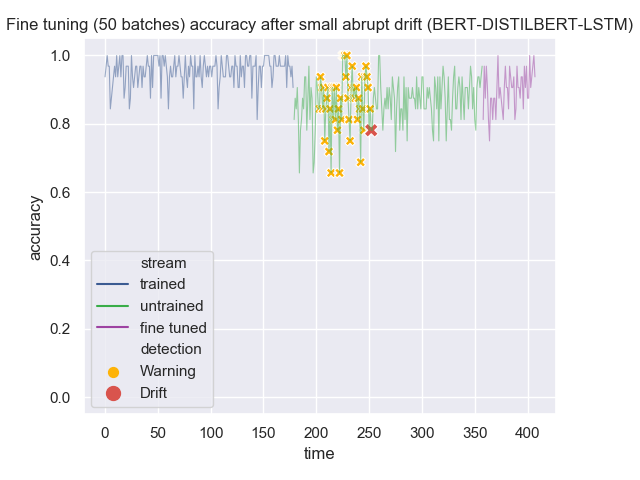
\includegraphics[width=0.8\linewidth]{assets/addressing-change/fine_tuning_lstm_wos_1_BERT_DISTILBERT_50_batches.png}
\caption{Fine tuning experiments using 50 batches}
\label{fig:fine50}
\end{figure}

\begin{figure}[ht!]
\centering
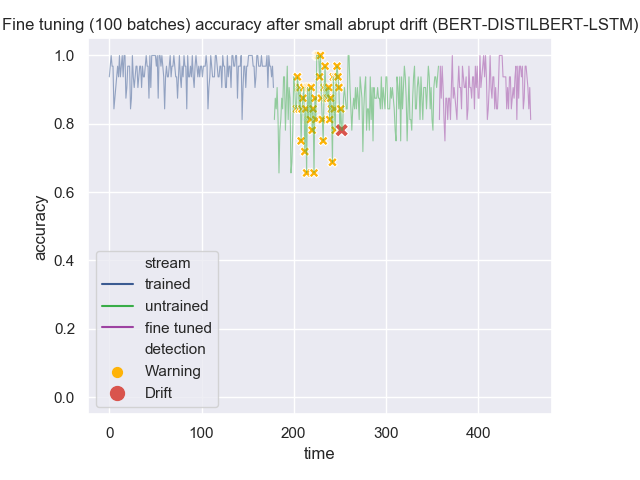
\includegraphics[width=0.8\linewidth]{assets/addressing-change/fine_tuning_lstm_wos_1_BERT_DISTILBERT_100_batches.png}
\caption{Fine tuning experiments using 100 batches}
\label{fig:fine100}
\end{figure}

TODO: also make and add results for a full epoch

TODO: might also want to create new pictures in which you run a fourth stream using already fine tuned network.

\subsection{Discussion}

Discussion on the fine tuning results.

\section{Mapping}

Maybe split this into two parts: Procrustes method and GAN method.

Explain the advantages of the Procrustes method: extremely fast, and the cons, not that reliable since it's a linear mapping. Then outline the assumption that the GAN method should be faster than retraining the whole model, and it's only worth using when that is the case.

The explain the methods used for mapping, both the Procrustes and the GAN.

Also talk about the created dataset and why it was needed.

\subsection{Experimental Setup}

Outline assumptions and decisions made in the mapping experiments.

\subsection{Results}

Show the results.

\begin{figure}[ht!]
\centering
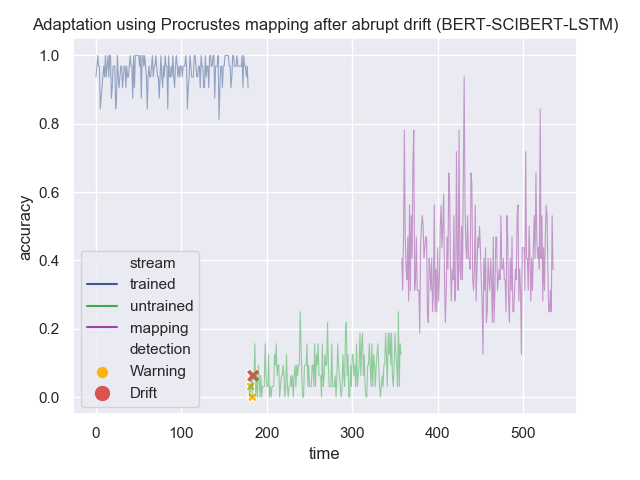
\includegraphics[width=0.8\linewidth]{assets/addressing-change/procrustes_lstm_wos_1_BERT_SCIBERT_5000_words_max.png}
\caption{Mapping using Procrustes method results using \textbf{max} embeddings aggregation in dataset}
\label{fig:proc-max}
\end{figure}

\begin{figure}[ht!]
\centering
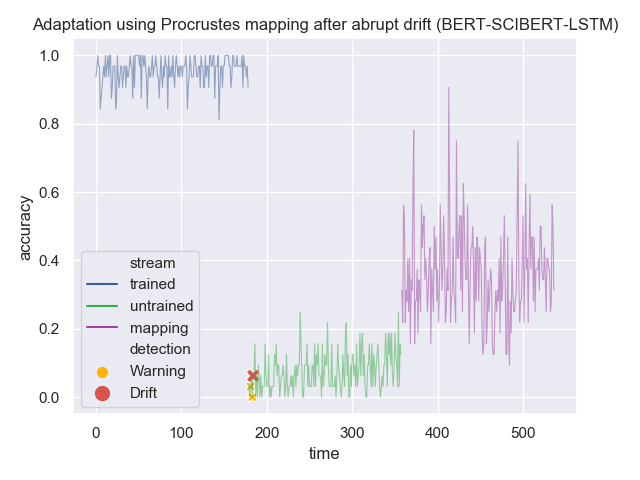
\includegraphics[width=0.8\linewidth]{assets/addressing-change/procrustes_lstm_wos_1_BERT_SCIBERT_5000_words_average.png}
\caption{Mapping using Procrustes method results using \textbf{average} embeddings aggregation in dataset}
\label{fig:proc-average}
\end{figure}

\begin{figure}[ht!]
\centering
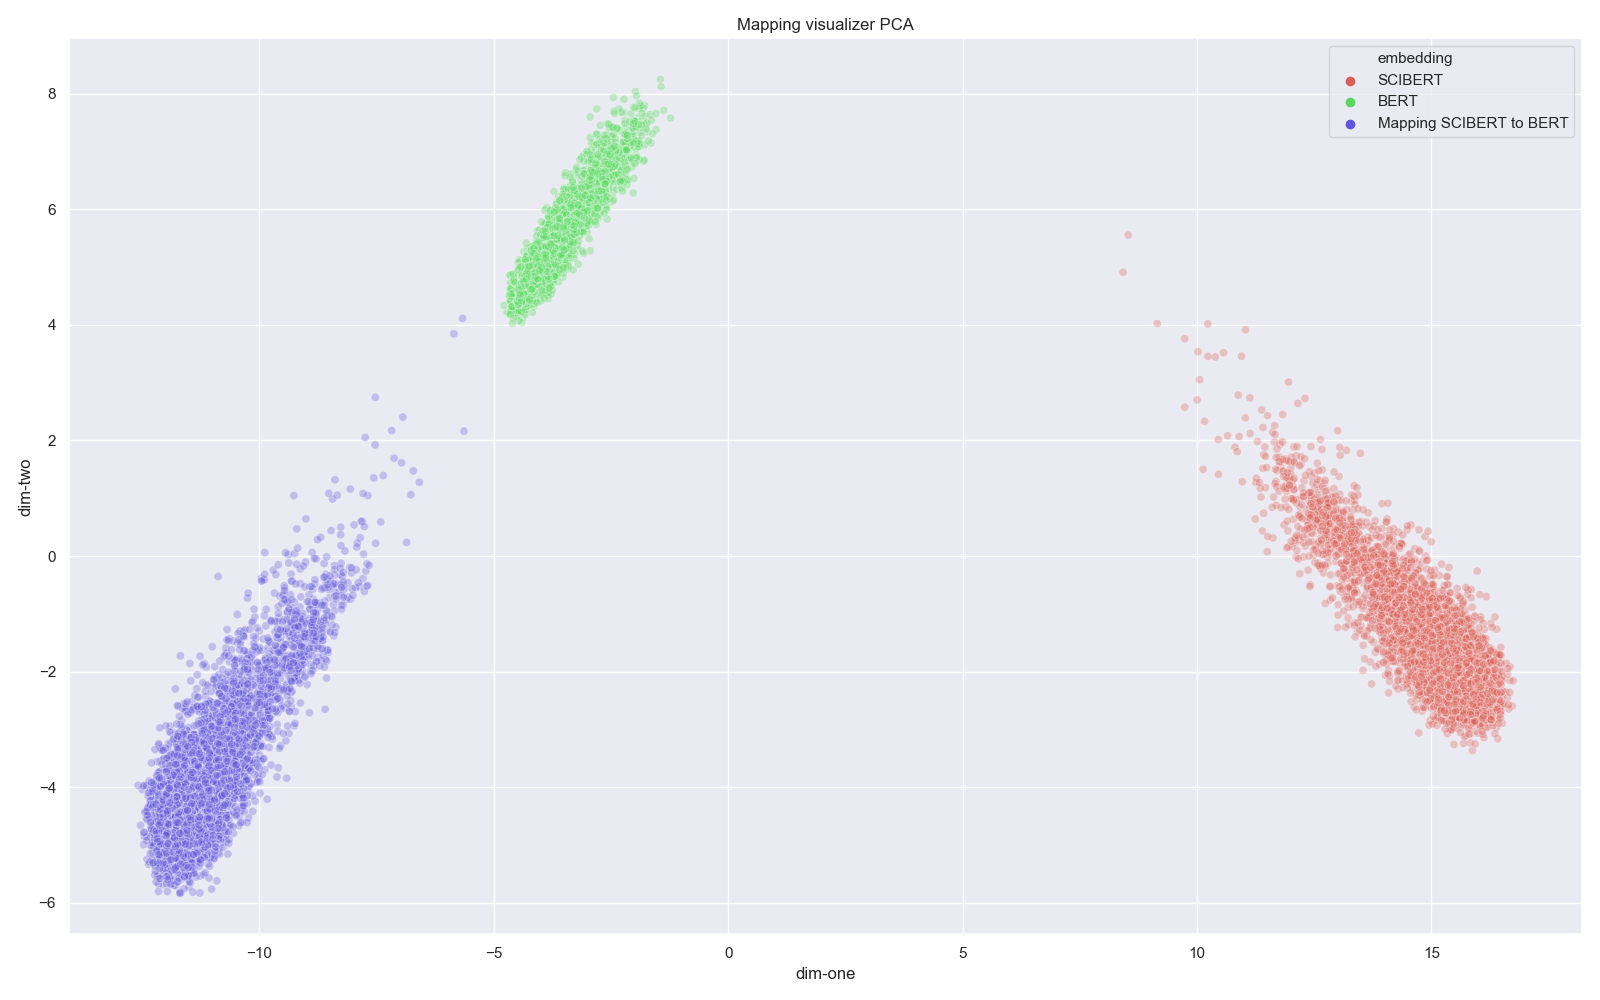
\includegraphics[width=0.8\linewidth]{assets/addressing-change/mapping_vis_pca_SCIBERT_BERT_average.png}
\caption{Embeddings spaces visualized using PCA for the Procrustes method}
\label{fig:proc-pca}
\end{figure}

\begin{figure}[ht!]
\centering
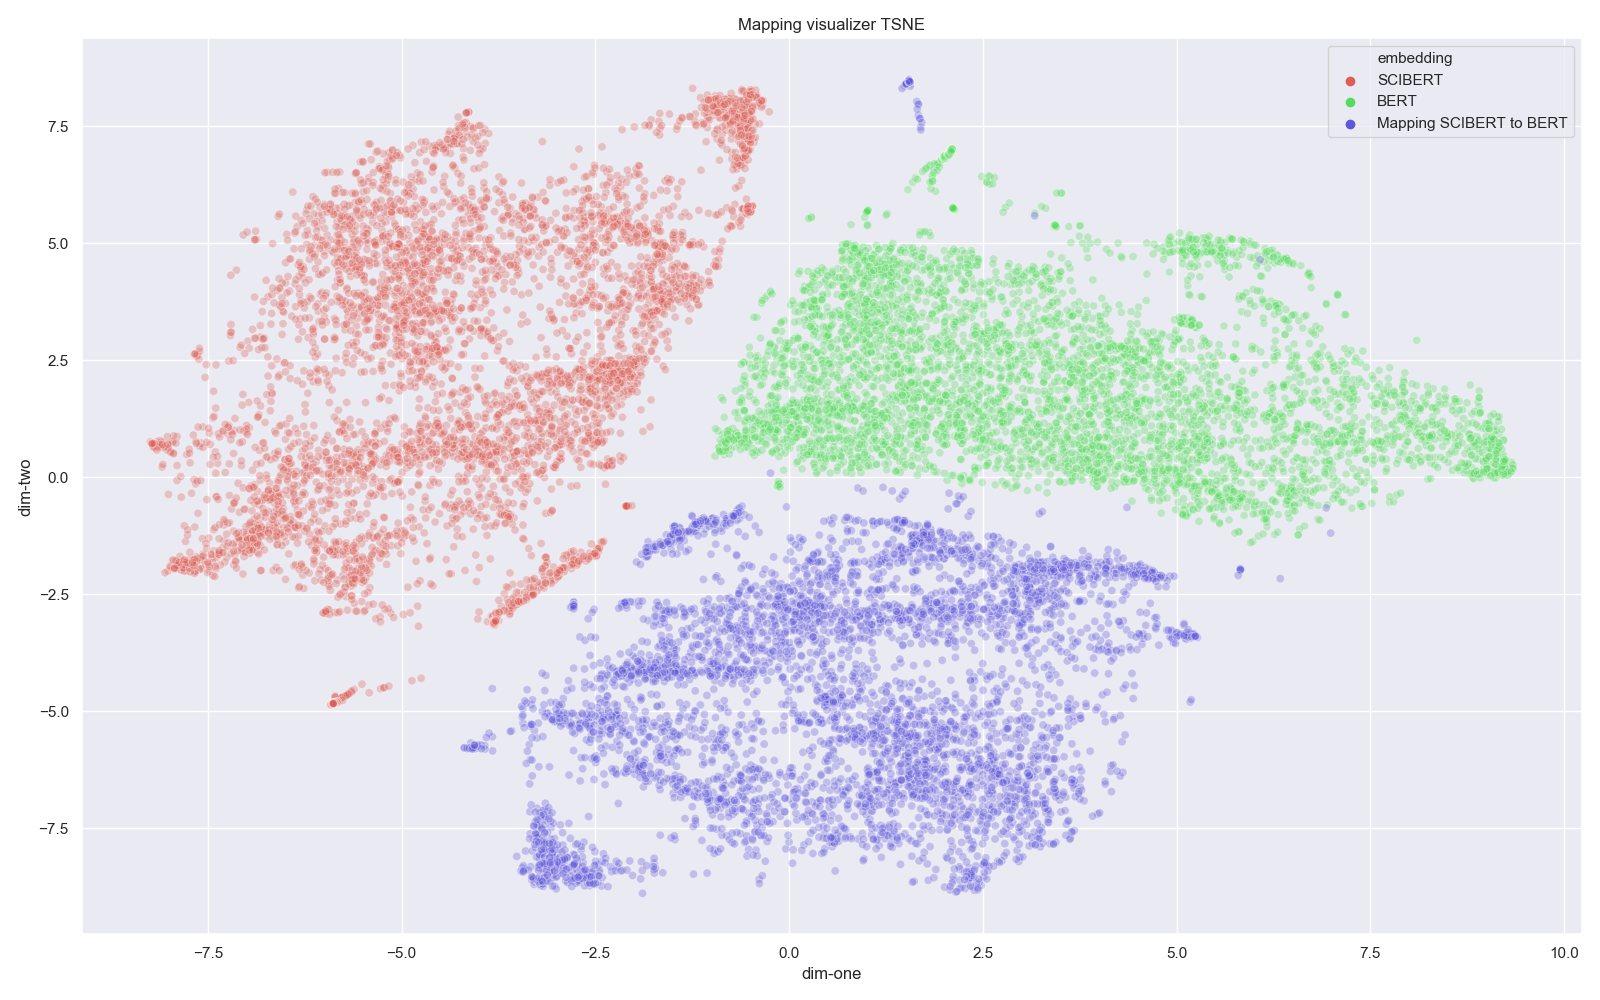
\includegraphics[width=0.8\linewidth]{assets/addressing-change/mapping_vis_tsne_SCIBERT_BERT_average.png}
\caption{Embeddings spaces visualized using t-SNE for the Procrustes method}
\label{fig:proc-tsne}
\end{figure}

\subsection{Discussion}

Discuss the results.

\chapter{Conclusion and Future Work}

\addcontentsline{toc}{chapter}{Bibliography}
\bibliographystyle{plainnat}
\bibliography{references.bib}

\end{document}

